\documentclass[runningheads]{llncs}
\usepackage[T1]{fontenc}
\usepackage{newtxtext}
\usepackage[varvw]{newtxmath}
\usepackage{amsmath,booktabs,array,tikz}
\usepackage{graphicx}
\usepackage[hidelinks,pdfusetitle,pdflang={en}]{hyperref}
\usetikzlibrary{arrows.meta}
\usepackage{pgfplots}
\pgfplotsset{compat=1.18}
\definecolor{routeLocal}{HTML}{295985}
\definecolor{routePublic}{HTML}{00766E}
\definecolor{routeSecure}{HTML}{AD4C20}
\newcommand{\Private}{\ensuremath{\mathsf{Private}}}
\newcommand{\Public}{\ensuremath{\mathsf{Public}}}
\newcommand{\Approved}{\ensuremath{\mathsf{Approved}}}
\newcommand{\Local}{\ensuremath{\mathsf{Local}}}
\newcommand{\MPC}{\ensuremath{\mathsf{MPC}}}
\newcommand{\PtwoP}{\ensuremath{\mathsf{P2P}}}
\newcommand{\J}{\mathcal{J}}
\newcommand{\Gt}{G_{\mathrm{task}}}
\newcommand{\Go}{G_{\mathrm{op}}}
\newcommand{\Gtnew}{G'_{\mathrm{task}}}
\newcommand{\srcA}{\textsc{PriGraph}}
\newcommand{\srcB}{\textsc{ShareRoute}}
\title{Cross-Layer Privacy Compilation for Decentralized LLM Inference}
\titlerunning{Cross-Layer Privacy Compilation}
\author{Anonymous Authors}
\authorrunning{Anonymous Authors}
\institute{Anonymous Institution}
\begin{document}
\maketitle
\begin{abstract}
Private language model serving on untrusted peers requires deciding what can
be disclosed and which residual operations need cryptographic protection.
We propose a cross-layer design that connects task graph rewriting to
operator-level information-flow analysis. Rewriting exposes reusable public
programs and retains private bindings on the client. Operator closure labels
the residual model graph and identifies subgraphs eligible for secure
multiparty computation (MPC). We evaluate the design on separately reported prototypes and controlled
benchmarks. In a CPU causal-attention diagnostic, changing private inputs
changes 2,133 positions that a token-only rule labels public. A pretrained
Pythia probe confirms that unchanged input tokens after a private field can
have changed output distributions. In a composed Pythia-70M forward, we execute the second layer's selected
attention scores and the final output projection with two-party workers.
On 96 synthetic prompts, all five policies preserve every constrained
FP32 choice. Relative to protecting all operands and returning the full
head, the joint policy reduces median attention openings from 430,080 to
77,824 bytes and output-head payload from 813,064 to 8,296 bytes.
A private candidate set retains full-head traffic. Separate arithmetic
and operator checks validate exact fixed-point computation. The composed
benchmark measures a local pipeline with two protected boundaries, with the
remaining Transformer operations executed on the trusted client.
\keywords{Decentralized inference \and Privacy \and Graph compilation \and MPC}
\end{abstract}

\section{Introduction}
Decentralized LLM-serving networks aggregate heterogeneous GPUs, but open participation makes prompt and activation privacy difficult: a peer receiving a private value in plaintext can retain or redistribute it. P2P model-serving platforms such as Petals and PlanetServe address access to compute \cite{petals,planetserve}; privacy-aware routing and plan caching address aspects of request placement and reuse \cite{ppmi,prism,apc}. Cryptographic private inference protects values but can multiply communication and latency, particularly for nonlinearity-intensive Transformers \cite{bolt,puma}.

The two source studies attack different layers of this cost. \srcA{} treats a \emph{reasoning task} as a typed DAG and changes \emph{what is computed}: produce a public, parameterized program once and perform private instantiation locally. \srcB{} treats a \emph{model execution} as an operator DAG and changes \emph{which operations require MPC}, and then \emph{how} secure computation runs. Combining these mechanisms suggests a principled ordering: \emph{rewrite away avoidable private computation before protecting the unavoidable remainder}. Crucially, this is not equivalent to concatenating two optimizers. The task-level rewrite changes the operator-level privacy footprint, while MPC cost changes whether a seemingly beneficial rewrite should be selected.

We describe a unified compilation interface with three legal execution paths: trusted local execution, public P2P execution of strictly public or approved data, and secure P2P execution on shares. Its optimization objective includes public generation/reuse, private MPC latency and bytes, WAN transfers, and quality loss. The planner treats disclosure legality as a feasibility constraint. The architecture is a \emph{proposed integration}; results from the two source prototypes remain independent. Our evaluation separates causal dependency, a matched arithmetic ablation and a protected output head driven by pretrained hidden states.

We specify a typed handoff from task rewriting to operator privacy closure and formulate joint planning under a fixed security stage. We examine the workload and trust assumptions behind each source result. Random and pretrained Transformers test causal dependency. Two-party executions test the composed arithmetic schedule, a candidate-restricted pretrained output head, and causal attention scores.

\section{Threat Model and Execution Semantics}
\paragraph{Participants and disclosure.}
A trusted device owns user context $X_u$ and controls all declassification. A P2P pool hosts open-weight public LLMs and possibly MPC parties. Public peers may inspect and record their received plaintext. The client has a planner, disclosure broker, local verifier, and secret-share encoder. We assume authenticated transport in deployment. Public peers can act adversarially. Weights are public; model-weight secrecy is outside scope. Timing, task shape, request length, and peer identities remain metadata leakage. Blockchain, if used, is a registration/staking substrate, never a place to store plaintext secrets or shares.

\paragraph{Privacy types and execution paths.}
A task node or operator edge is typed by schema and sensitivity $\ell\in\{\Public,\Approved,\Private\}$. The $\Approved$ label is allowed only for a named, user-authorized egress field; it is \emph{not} inferred by the optimizer. Join propagation makes any result private when it depends on undisclosed private values. A node executes (1) \Local{} on the trusted device, (2) public $\PtwoP$ in plaintext only on $\Public$ or explicitly $\Approved$ values, or (3) $\MPC$ on secret shares. Private values in a share-based path are never reconstructed on public peers. A public key identifying a cached artifact must be derived exclusively from approved/public properties; a key constructed from private bindings would be a secret-dependent side channel.

\paragraph{Cryptographic stages.}
We retain the original non-mixable stage taxonomy: S0 is trusted local execution, with no cryptographic protection claim; S1 is semi-honest 2PC, whose parties follow the protocol but may inspect their own views; S2 is semi-honest honest-majority 3PC for the reported replicated-ring backend, with at most one corrupt party; S3 is actively secure MPC requiring a separately validated backend. S1 and S2 differ in security assumptions, and performance figures across them must be labeled as such. Independent trust domains and corruption bounds are assumptions, not empirically demonstrated Sybil resistance.

\section{Hierarchical Privacy Graph Compiler}
The reasoning compiler first generates a typed task DAG $\Gt=(V_t,E_t)$. Each node has an operation, input/output schemas, sensitivity, capability requirements, cost profile, and optional executable validator. An admissible typed rewrite produces $\Gtnew\in\mathcal{R}(\Gt)$; the operator compiler then traces the selected LLM invocations into $\Go=(V_o,E_o)$ and links each invocation's inputs to task-graph outputs. The joined plan retains edge provenance from both layers. Figure~\ref{fig:arch} distinguishes compilation stages and runtime paths.

\begin{figure}[t]
\centering
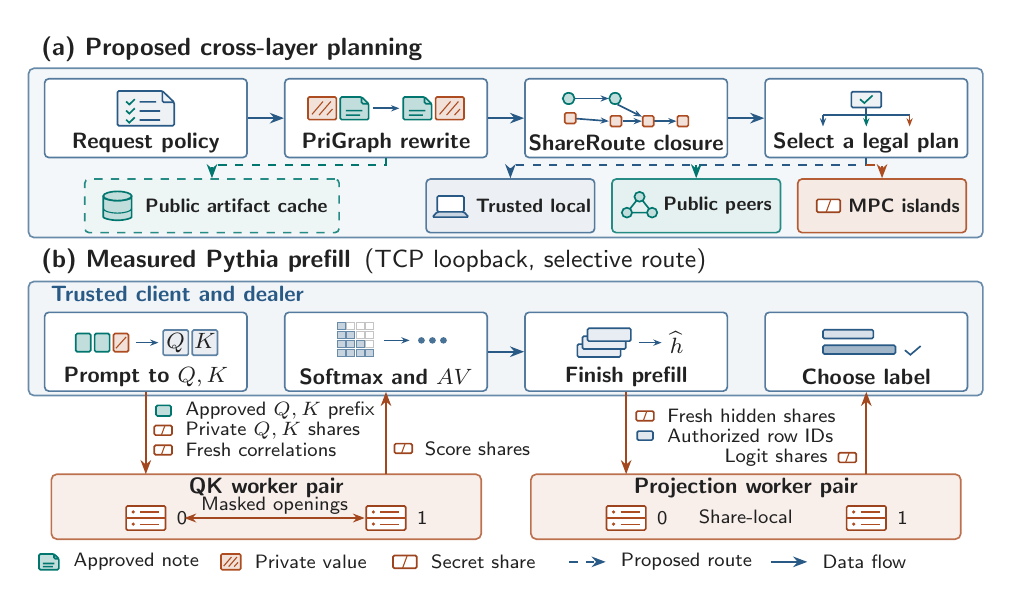
\begin{tikzpicture}[
  x=1cm,y=.96cm,
  font=\sffamily\fontsize{8}{9.3}\selectfont,
  ink/.style={text=black!87},
  panel/.style={anchor=west,ink,font=\sffamily\bfseries\fontsize{9}{10}\selectfont},
  detail/.style={ink,font=\sffamily\fontsize{7.3}{8.5}\selectfont},
  tile/.style={rounded corners=1.5pt,semithick,align=center,ink,inner sep=2pt},
  stage/.style={tile,draw=routeLocal!80,fill=white,text width=2.43cm,minimum height=10mm},
  stage label/.style={ink,font=\sffamily\bfseries\fontsize{8}{9.3}\selectfont},
  route tile/.style={tile,minimum height=6.8mm,minimum width=2.14cm},
  route label/.style={stage label,anchor=west,inner sep=1pt,
                       font=\sffamily\bfseries\fontsize{7.3}{8.5}\selectfont},
  glyph/.style={semithick,draw=routeLocal,rounded corners=.5pt},
  approved/.style={glyph,draw=routePublic,fill=routePublic!24},
  private/.style={glyph,draw=routeSecure,fill=routeSecure!17},
  share/.style={glyph,draw=routeSecure!90!black,fill=white},
  flow/.style={semithick,-{Stealth[length=1.8mm]},draw=routeLocal},
  plan/.style={flow,dashed},
  wire/.style={flow,draw=routeSecure!94!black},
  micro flow/.style={flow,-{Stealth[length=1.05mm]}},
  pics/note/.style={code={
    \draw[approved] (-.18,-.15) -- (-.18,.15) -- (.09,.15) -- (.18,.06) -- (.18,-.15) -- cycle;
    \draw[glyph,draw=routePublic] (.09,.15) |- (.18,.06) (-.11,-.03) -- (.10,-.03) (-.11,-.09) -- (.07,-.09);
  }},
  pics/value/.style={code={
    \draw[private] (-.18,-.15) rectangle (.18,.15);
    \draw[routeSecure,thin] (-.13,-.08) -- (.01,.09) (-.04,-.09) -- (.11,.09) (.06,-.09) -- (.13,-.01);
  }},
  pics/share/.style={code={
    \draw[share] (-.15,-.085) rectangle (.15,.085);
    \draw[routeSecure,thin] (-.03,-.085) -- (.03,.085);
  }},
  pics/rack/.style={code={
    \draw[share] (-.25,-.16) rectangle (.25,.16);
    \draw[routeSecure,thin] (-.25,0) -- (.25,0) (-.07,.08) -- (.17,.08) (-.07,-.08) -- (.17,-.08);
    \fill[routeSecure] (-.16,.08) circle (.023) (-.16,-.08) circle (.023);
  }}]

\node[panel] at (.04,0) {(a) Proposed cross-layer planning};
\draw[rounded corners=2pt,semithick,draw=routeLocal!70,fill=routeLocal!5]
  (0,-.25) rectangle (12.12,-2.49);
\node[stage] (request) at (1.49,-.91) {};
\node[stage] (rewrite) at (4.54,-.91) {};
\node[stage] (closure) at (7.59,-.91) {};
\node[stage] (choose) at (10.64,-.91) {};
\draw[flow] (request) -- (rewrite);
\draw[flow] (rewrite) -- (closure);
\draw[flow] (closure) -- (choose);
\node[stage label] at (1.49,-1.24) {Request policy};
\node[stage label] at (4.54,-1.24) {PriGraph rewrite};
\node[stage label] at (7.59,-1.24) {ShareRoute closure};
\node[stage label] at (10.64,-1.24) {Select a legal plan};

\begin{scope}[shift={(1.49,-.78)}]
  \draw[glyph,fill=routeLocal!8] (-.36,-.23) -- (-.36,.23) -- (.21,.23) -- (.36,.08) -- (.36,-.23) -- cycle;
  \draw[glyph] (.21,.23) |- (.36,.08) (-.08,.085) -- (.13,.085) (-.08,-.035) -- (.18,-.035) (-.08,-.155) -- (.18,-.155);
  \draw[routePublic,semithick] (-.25,.09) -- (-.21,.05) -- (-.14,.12)
    (-.25,-.03) -- (-.21,-.07) -- (-.14,0) (-.25,-.15) -- (-.21,-.19) -- (-.14,-.12);
\end{scope}
\pic at (3.73,-.78) {value};
\pic at (4.14,-.78) {note};
\draw[micro flow] (4.37,-.78) -- (4.71,-.78);
\pic at (4.94,-.78) {note};
\pic at (5.35,-.78) {value};
\begin{scope}[shift={(7.59,-.79)}]
  \draw[micro flow] (-.65,.14) -- (-.22,.14);
  \draw[micro flow] (-.71,-.12) -- (-.22,-.16);
  \draw[micro flow] (-.11,.06) -- (.20,-.10);
  \draw[micro flow] (-.04,-.16) -- (.20,-.16);
  \draw[micro flow] (.36,-.16) -- (.64,-.16);
  \draw[approved] (-.73,.14) circle (.075) (-.14,.14) circle (.075);
  \draw[private] (-.78,-.19) rectangle (-.64,-.05)
    (-.20,-.23) rectangle (-.06,-.09) (.21,-.23) rectangle (.35,-.09)
    (.65,-.23) rectangle (.79,-.09);
\end{scope}
\begin{scope}[shift={(10.64,-.78)}]
  \draw[glyph,fill=routeLocal!8] (-.19,.22) rectangle (.19,.01);
  \draw[routePublic,semithick] (-.08,.12) -- (-.025,.07) -- (.08,.17);
  \draw[glyph] (0,.01) -- (0,-.09) (-.55,-.09) -- (.55,-.09);
  \draw[micro flow] (-.55,-.09) -- (-.55,-.24);
  \draw[micro flow,draw=routePublic] (0,-.09) -- (0,-.24);
  \draw[micro flow,draw=routeSecure] (.55,-.09) -- (.55,-.24);
\end{scope}

\node[route tile,draw=routePublic!85,dashed,fill=routePublic!7,minimum width=3.23cm]
  (cache) at (2.33,-2.07) {};
\node[route tile,draw=routeLocal!80,fill=routeLocal!9] (local) at (6.12,-2.07) {};
\node[route tile,draw=routePublic!85,fill=routePublic!10] (public) at (8.48,-2.07) {};
\node[route tile,draw=routeSecure!90,fill=routeSecure!12] (islands) at (10.84,-2.07) {};
\draw[plan,draw=routePublic] (rewrite.south) -- (4.54,-1.53) -| (cache.north);
\draw[plan] (choose.south) -- (10.64,-1.53) -| (local.north);
\draw[plan,draw=routePublic] (8.48,-1.53) -- (public.north);
\draw[plan,draw=routeSecure] (10.64,-1.53) -| (islands.north);
\begin{scope}[shift={(1.13,-2.07)}]
  \draw[approved] (-.18,.13) arc (180:360:.18 and .061) -- (.18,-.13)
    arc (0:-180:.18 and .061) -- cycle;
  \draw[approved] (0,.13) ellipse (.18 and .061);
  \draw[routePublic,thin] (-.18,-.035) arc (180:360:.18 and .061);
\end{scope}
\node[route label] at (1.44,-2.07) {Public artifact cache};
\begin{scope}[shift={(5.36,-2.07)}]
  \draw[glyph,fill=white] (-.17,-.08) rectangle (.17,.13);
  \draw[glyph,fill=routeLocal!25] (-.17,-.08) -- (-.23,-.15) -- (.23,-.15) -- (.17,-.08) -- cycle;
\end{scope}
\node[route label] at (5.64,-2.07) {Trusted local};
\begin{scope}[shift={(7.76,-2.07)}]
  \draw[routePublic,semithick] (-.16,-.09) -- (0,.12) -- (.16,-.09) -- cycle;
  \draw[approved] (-.16,-.09) circle (.065) (0,.12) circle (.065) (.16,-.09) circle (.065);
\end{scope}
\node[route label] at (8.02,-2.07) {Public peers};
\pic at (10.16,-2.07) {share};
\node[route label] at (10.37,-2.07) {MPC islands};

\node[panel] at (.04,-2.81) {(b) Measured Pythia prefill\enspace\mdseries (TCP loopback, selective route)};
\draw[rounded corners=2pt,semithick,draw=routeLocal!70,fill=routeLocal!6]
  (0,-3.07) rectangle (12.12,-4.58);
\node[stage label,anchor=west,text=routeLocal] at (.16,-3.24) {Trusted client and dealer};
\node[stage] (qkInput) at (1.49,-4.00) {};
\node[stage] (qkOutput) at (4.54,-4.00) {};
\node[stage] (hidden) at (7.59,-4.00) {};
\node[stage] (label) at (10.64,-4.00) {};
\draw[flow] (qkOutput) -- (hidden);
\node[stage label] at (1.49,-4.33) {Prompt to $Q,K$};
\node[stage label] at (4.54,-4.33) {Softmax and $AV$};
\node[stage label] at (7.59,-4.33) {Finish prefill};
\node[stage label] at (10.64,-4.33) {Choose label};

\begin{scope}[shift={(1.49,-3.88)}]
  \foreach \i in {0,1} {\draw[approved] ({-.89+.24*\i},-.12) rectangle ++(.19,.24);}
  \draw[private] (-.41,-.12) rectangle ++(.19,.24);
  \draw[routeSecure,thin] (-.38,-.075) -- (-.25,.075);
  \draw[micro flow] (-.13,0) -- (.16,0);
  \foreach \x/\qkLabel in {.38/Q,.75/K} {
    \draw[glyph,draw=routeLocal!75,fill=routeLocal!10]
      (\x,0) ++(-1.6mm,-1.6mm) rectangle ++(3.2mm,3.2mm);
    \node[stage label,inner sep=0pt,text height=1.55ex,text depth=.5ex]
      at (\x,0) {$\qkLabel$};
  }
\end{scope}
\begin{scope}[shift={(4.54,-3.85)}]
  \foreach \row in {0,...,3} {\foreach \col in {0,...,3} {
    \ifnum\col>\row
      \draw[black!23,line width=.25pt] ({-.62+.12*\col},{.245-.12*\row}) rectangle ++(.10,-.10);
    \else
      \draw[routeLocal!70,fill=routeLocal!26,line width=.25pt]
        ({-.62+.12*\col},{.245-.12*\row}) rectangle ++(.10,-.10);
    \fi
  }}
  \draw[micro flow] (-.02,0) -- (.30,0);
  \foreach \i in {0,1,2} {\fill[routeLocal!85] ({.45+.14*\i},0) circle (.043);}
\end{scope}
\begin{scope}[shift={(7.59,-3.88)}]
  \foreach \i in {0,1,2} {
    \draw[glyph,fill=routeLocal!11] ({-.62+.065*\i},{-.19+.105*\i})
      rectangle ++(.55,.17);
  }
  \draw[micro flow] (.16,0) -- (.45,0);
  \node[stage label] at (.64,0) {$\widehat{h}$};
\end{scope}
\begin{scope}[shift={(10.64,-3.89)}]
  \draw[glyph,fill=routeLocal!18] (-.55,.065) rectangle (.09,.18);
  \draw[glyph,fill=routeLocal!44] (-.55,-.14) rectangle (.37,-.025);
  \draw[routeLocal,semithick] (.49,-.09) -- (.56,-.15) -- (.69,-.035);
\end{scope}

\draw[rounded corners=2pt,semithick,draw=routeSecure!80,fill=routeSecure!9]
  (.29,-5.62) rectangle (5.75,-6.48);
\draw[rounded corners=2pt,semithick,draw=routeSecure!80,fill=routeSecure!9]
  (6.38,-5.62) rectangle (11.84,-6.48);
\node[stage label] at (3.02,-5.80) {QK worker pair};
\node[stage label] at (9.11,-5.80) {Projection worker pair};
\foreach \x/\p in {1.49/0,4.54/1,7.59/0,10.64/1} {
  \pic at (\x,-6.20) {rack};
  \node[detail,anchor=west] at ({\x+.27},-6.20) {\p};
}
\draw[semithick,draw=routeSecure!94!black,{Stealth[length=1.5mm]}-{Stealth[length=1.5mm]}]
  (1.98,-6.20) -- node[detail,above,inner sep=1pt] {Masked openings} (4.27,-6.20);
\node[detail] at (9.11,-6.18) {Share-local};

\draw[wire] (qkInput.south) -- (1.49,-5.62);
\draw[wire] (4.54,-5.62) -- (qkOutput.south);
\draw[wire] (hidden.south) -- (7.59,-5.62);
\draw[wire] (10.64,-5.62) -- (label.south);
\draw[approved] (1.62,-4.85) rectangle ++(.19,.14);
\node[detail,anchor=west] at (1.87,-4.78) {Approved $Q,K$ prefix};
\pic[scale=.75] at (1.71,-5.04) {share};
\node[detail,anchor=west] at (1.87,-5.04) {Private $Q,K$ shares};
\pic[scale=.75] at (1.71,-5.30) {share};
\node[detail,anchor=west] at (1.87,-5.30) {Fresh correlations};
\pic[scale=.75] at (4.76,-5.28) {share};
\node[detail,anchor=west] at (4.91,-5.28) {Score shares};
\pic[scale=.75] at (7.83,-4.85) {share};
\node[detail,anchor=west] at (7.99,-4.85) {Fresh hidden shares};
\draw[glyph,fill=routeLocal!14] (7.73,-5.17) rectangle ++(.20,.12);
\node[detail,anchor=west] at (7.99,-5.11) {Authorized row IDs};
\pic[scale=.75] at (10.40,-5.40) {share};
\node[detail,anchor=east] at (10.27,-5.40) {Logit shares};

\pic[scale=.7] at (.26,-6.78) {note};
\node[detail,anchor=west] at (.45,-6.78) {Approved note};
\pic[scale=.7] at (2.57,-6.78) {value};
\node[detail,anchor=west] at (2.75,-6.78) {Private value};
\pic at (4.78,-6.78) {share};
\node[detail,anchor=west] at (4.99,-6.78) {Secret share};
\draw[plan] (6.87,-6.78) -- (7.33,-6.78);
\node[detail,anchor=west] at (7.40,-6.78) {Proposed route};
\draw[flow] (9.43,-6.78) -- (9.89,-6.78);
\node[detail,anchor=west] at (9.96,-6.78) {Data flow};
\end{tikzpicture}

\caption{Task rewriting exposes reusable public programs before operator
closure identifies secure subgraphs. Dashed arrows assign work to execution
domains. Solid arrows indicate compilation flow or results returned to the client.}
\label{fig:arch}
\end{figure}

\subsection{Task-Layer Rewriting and Canonicalization}
We preserve the three \srcA{} rewrite operators and their conditions:
\begin{itemize}
\item \emph{Separate-Template} replaces a separable mixed node with a public program generator and a local private-binding node.
\item \emph{Lift-Public-Subgraph} replaces a recognized canonical rule with a parameterized public artifact, keyed by rule/version and instantiated locally on private values; the public model returns a \emph{program}, not a user-specific answer.
\item \emph{Late-Private-Fusion} extracts the public prefix of a mixed computation and defers the private combination to one final local fusion node.
\end{itemize}
A rewrite is admitted only with (i) legal information flow, (ii) an executable regression contract for deterministic steps or an empirical quality bound and local fallback for free-form steps, and (iii) typed, versioned interfaces for shareable nodes. PriGraph uses beam search over rewrites and an inner placement/cache planner (MILP on small cases). If no safe rewrite succeeds, it executes the original graph locally.

A reusable artifact is a tuple of a parameterized program, typed inputs and outputs, assumptions, region, version, content hash, and validator. Strong schema, region, version, and assumption checks are required for safe cache hits; semantic similarity alone yields only a candidate for local verification. Creation occurs during graph rewriting, not after the first task completes. Expected reuse benefit is $R_{\mathrm{reuse}}=\sum_{a\in A(\Gtnew)}p_a[c_{\mathrm{gen}}(a)-c_{\mathrm{fv}}(a)]$. Artifacts must not contain private values or per-session MPC masks/triples.

\subsection{Operator-Level Closure and Secure Islands}
For a model call that consumes protected activations, tracing PyTorch/ONNX operations yields an operator graph with linear projections, QK/AV products, normalization, Softmax, FFN, and optional routing. \srcB{} performs forward private-taint propagation and a backward consistency pass. Every unauthorized path from a private tensor to a non-MPC remote endpoint is rejected. A \emph{secure island} is a connected subgraph executed under MPC. Island boundaries are chosen jointly with conversion, round-trip, and share-lifecycle costs: a collection of smaller islands is not necessarily cheaper than one contiguous region. Shares persist across secure steps; plaintext reconstruction occurs only at the trusted client or an explicitly approved release point.

The protocol-aware backend distinguishes linear operations on public weights (share-local arithmetic) from expensive nonlinearities requiring online interaction. It may fuse groups of operations, schedule Beaver-triple preprocessing offline, or optimize KV-cache handling. Protocol fusion and trust-aware cohort placement are \emph{design capabilities} of the source study, not separately experimentally validated speedups. In autoregressive generation, private-token attention can depend on public-prefix keys without allowing the compiler to relabel private hidden states as public; privacy closure governs every tensor.

\subsection{The Cross-Layer Interface}
Each edge records its schema, privacy label, origin, authorization, and contract. Each LLM call exposes its approved public prefix, residual private inputs, whether local evaluation is possible, and a cryptographic fallback stage. An operator's taint is calculated \emph{after} the candidate task rewrite. Consequently, $\Gtnew$ changes the amount of secure work; MPC prices can in turn affect which task rewrite is optimal. We define three boundary checks: \emph{(B1)} no public node consumes private plaintext or a secret-derived cache key; \emph{(B2)} every remote private operator lies in a legally composed MPC island, with shares preserved; \emph{(B3)} outputs are reconstructed or disclosed only at policy-approved endpoints. These conditions are necessary; they do not eliminate metadata leakage or guarantee a correct compiler implementation.

\paragraph{Causal-attention dependence.}
For a standard \emph{dense causal} decoder that mixes all earlier positions, let $s_i=1$ when the input to the remote model at position $i$ contains an undisclosed private value. A conservative privacy-closure label for a hidden state at position $t$ is
\begin{equation}\label{eq:prefix}
  q_t=\bigvee_{i\leq t}s_i,\qquad
  F_{\rm safe}=\frac{1}{L}\sum_{t=1}^{L}(1-q_t).
\end{equation}
Consequently, an approved public \emph{suffix} that follows private text is not automatically safe for plaintext execution: its hidden states can depend on earlier secrets. A public prefix followed by a private suffix is different. This conservative dependency rule depends on causal dense attention; explicit architectural block sparsity or correctly justified declassification may alter it. The rewrite compiler can change the $s_i$ actually presented to each model invocation, so task-level decisions must precede operator-level closure. For $k$ uniformly
placed private positions among $L$ tokens, the $k+1$ public gaps are
exchangeable and sum to $L-k$. The expected public prefix length is therefore
$(L-k)/(k+1)$, giving $F_{\rm safe}=15\%$ in expectation at $L=16,k=4$.

\paragraph{Compilation order and rejection.}
For each task rewrite candidate $r$, the proposed compiler must (1) check that public outputs derive only from policy-approved inputs; (2) compute the program hash, version, region, and validator preconditions; (3) trace the model calls remaining after local binding; (4) compute operator taint and permissible secure islands; and (5) score the plan only among protocols satisfying one fixed adversary stage. A failed executable contract, poisoned artifact, unsafe declassification, missing MPC cohort, or violated numerical tolerance rejects that candidate, rather than lowering its safety requirements. This order also clarifies a non-goal: secret-sharing inputs to a Transformer cannot be replaced by a public prompt merely because their \emph{task schema} is public.

\section{Compositional Planning and Security}
\subsection{Joint Cost Model}
A plan $z=(\Gtnew,\pi,\kappa,S,p,\rho,m,b)$ selects a rewritten task graph, task placements $\pi$, cache actions $\kappa$, secure islands $S$, per-island MPC protocols $p$, cohorts/peer routes $\rho$, weight layout $m$, and offline budget $b$. A proposed cross-layer objective is
\begin{equation}\label{eq:obj}
\begin{aligned}
\min_{z\in\mathcal{F}_s}\;\J_s(z)={}&\mathbb{E}[T_{\rm critical}^{\rm online}]
+\lambda B_{\rm WAN}^{\rm online}+\mu C_{\rm GPU}\\
&+\eta\,T_{\rm offline}^{\rm amort.}+\xi M_{\rm peak}
+\nu L_{\rm quality}-\gamma R_{\rm reuse},
\end{aligned}
\end{equation}
where $\mathcal{F}_s$ requires information-flow legality, valid rewrite contracts, an acceptable quality bound, protocol correctness under \emph{fixed} security stage $s$, per-peer capacity, and safe preprocessing. We do not compare minima across security stages as if they had equivalent threat models. The original task optimizer used latency, GPU-seconds, WAN bytes, and quality loss; the original MPC optimizer used online critical path, online bytes, amortized offline time, memory, and quality. Equation~\eqref{eq:obj} is their \emph{proposed} integration, not an experimentally calibrated cross-layer objective.

\paragraph{Search and fallback.}
The compiler enumerates admissible task rewrites, validates reusable public artifacts, traces the required model calls, and calculates operator closure for each candidate. Within each fixed security stage it searches plans over islands, protocols, cohorts, and layouts and scores the resulting end-to-end critical path including task-planner overhead. For small cases one can use a mixed-integer formulation; for larger cases a beam over rewrites with a layered operator planner is more plausible. If a private task cannot be decomposed, the proposed framework may still choose \emph{secure MPC} for the private remainder \emph{provided} a valid security-stage cohort is available, otherwise trusted local execution. This extends the source \srcA{} fallback; it is a design proposal, not a measured behavior.

\subsection{Confidentiality Argument and Its Boundary}
\textbf{Claim (conditional plaintext non-egress).} Assume every selected task rewrite preserves policy-labeled data dependencies; every public artifact key is independent of non-approved private bindings; the operator closure and island partition satisfy B1--B3; and each MPC backend realizes its stated security under the declared corruption model. Then no unauthorized private plaintext can be delivered to a public execution endpoint. \emph{Argument.} Binding on the client retains privacy labels on any private-dependent result. Only a policy-approved disclosure rule may release that result. Public payloads and cache keys must also account for control dependencies. Forward privacy closure prevents non-approved private-descendant tensors from entering public P2P. For every remaining off-device private computation, shares enter an MPC island and are never reconstructed on public peers, except as explicitly authorized. Sequential secure protocol composition establishes cryptographic confidentiality only under the chosen stage's corruption bound \cite{canetti}. This is a modular proof sketch, \emph{not} formal verification of the integrated compiler or an implementation-level security proof.

The guarantee excludes task-pattern and timing leakage, network anonymity, unproven party independence, side channels, malicious deviations under semi-honest protocols, failure-time privacy, and quality preservation of unrestricted free-form reasoning. If the cryptographic assumptions cannot be met, the scheduler must reject that remote plan rather than silently fall back to plaintext.

\section{Evidence from the Two Source Prototypes}
\label{sec:eval}
These results come from \srcA{}~\cite{prigraph-source} and
\srcB{}~\cite{shareroute-source}. The source prototypes have distinct
models, workloads and protocols.

\subsection{Task Rewriting, Reuse, and Planning (PriGraph)}
On 360 synthetic, verifiable tasks, four seed blocks of 30 per family cover numerical payroll, event-log memory, and code-generation-with-private-constant tasks. The local role uses Qwen2.5-7B-Instruct; a public role uses Qwen2.5-14B-Instruct (greedy decoding). The unrewritten 14B remote arm is a \emph{privacy-violating diagnostic}, not a legal deployment. Table~\ref{tab:task} keeps the original three-arm control: the rewritten arm uses a public program generator and deterministic local binding; 360/360 graphs passed the static information-flow checker.

\begin{table}[t]
\centering\caption{Original PriGraph accuracy on 360 synthetic tasks/arm. Overall 95\% bootstrap CIs: A [49.2, 59.4], B [64.4, 73.9]. B violates the privacy requirement.}\label{tab:task}
\small\renewcommand{\arraystretch}{1.15}
\begin{tabular}{@{}p{4.4cm}rrrr@{}}\toprule
Arm & Overall (\%) & Numerical (\%) & Memory (\%) & Coding (\%) \\ \midrule
A: original task, 7B local & 54.2 & 62.5 & 100.0 & 0.0 \\
B: original task, 14B remote & 69.2 & 80.8 & 100.0 & 26.7 \\
C: rewritten, 14B public + local & \textbf{100.0} & 100.0 & 100.0 & 100.0 \\
\bottomrule\end{tabular}
\end{table}

Tool-augmented local 7B also reached 100\% on the 400 explicit-formula
tasks. Its 38\% on 200 implicit-formula tasks has no matched rewrite
arm. The private-formula experiment recorded 104/104 local fallbacks.
Source simulations report up to 12-to-2 fewer program generations
and planning objectives 24.4\% and 165.0\% higher than joint for two
sequential schedules. They compare task-layer policies under calibrated
costs, whereas the proposed cross-layer objective remains unevaluated.

\subsection{Secure Islands and MPC Backends (ShareRoute)}
The MPC source uses GPT-2 125M for plaintext baselines and operator-DAG analysis, and real MP-SPDZ on a \emph{$d=32$, 2-layer mini-GPT} (vocabulary 64, sequence length 16) for performance. Semi2k 2PC and replicated-ring 3PC are measured on a single-machine LAN. It reports 9,800 operator comparisons and 120/120 end-to-end argmax agreement; these are functional correctness checks, not proof of cryptographic implementation security or full-scale LLM task utility. Source data are synthetic.

\begin{table}[t]\centering\caption{Original ShareRoute mini-GPT 2PC workload sweep as reported by the source. Time is MPC time (five seeds, mean $\pm$ SD). Communication is per party.}\label{tab:sweep}\small
\begin{tabular}{@{}rrrrr@{}}\toprule
Public fraction & Time (s) & Comm. (MB) & Time / full & Bytes / full \\ \midrule
0\% (full MPC) & $73.9\pm0.8$ & 6313 & 1.00 & 1.00 \\
25\% & $55.5\pm0.8$ & 4783 & 0.75 & 0.76 \\
50\% & $38.2\pm0.5$ & 3222 & 0.52 & 0.51 \\
75\% & $19.5\pm0.1$ & 1629 & 0.26 & 0.26 \\
100\% & 0 & 0 & 0 & 0 \\
\bottomrule\end{tabular}
\end{table}

At 75\% public input, the source sweep reports 19.5 seconds and
1,629 MB per party versus 73.9 seconds and 6,313 MB at 0\% public input,
under the same 2PC stage. This is a workload sensitivity comparison. An
island-selection speedup requires both arms to process the same prompt,
public positions, policy, and protocol. Zero in the 100\%-public row is
zero MPC work. Ordinary GPU and end-to-end serving time remain outside
that row. When no relevant activations qualify for public execution, the
whole model remains in MPC. The source reports a compiler timeout at
$d=128$.

\section{CPU Diagnostic: Where Secrets Contaminate Causal Attention}\label{sec:cpu}
\paragraph{Question and implementation.}
Does labeling only the \emph{secret token positions} correctly identify the states that must be kept out of plaintext P2P execution? We ran a CPU diagnostic using PyTorch 2.10 and reproduced its counts on Apple Silicon with PyTorch 2.8: a randomly initialized, frozen, two-layer causal Transformer ($d=32$, four heads, FFN width 64, sequence length 16). It uses dense masked self-attention, LayerNorm and GELU; \emph{it is not the pretrained GPT-2 or cryptographic mini-GPT used by ShareRoute}. We varied the 0/25/50/75/100\% private-input fractions and three secret placements (prefix, suffix, uniformly sampled interleaving). With four model seeds and 12 perturbations/cell, this yields $5\times3\times4\times12=720$ paired input executions. Each pair changes only secret-position vectors; 16 output states are compared per pair. The source and raw per-case CSV are included in the repository, along with the command to repeat the test.

\paragraph{Results.}
The first secret fixes the public prefix under dense causal attention. Across 11,520 comparisons, every state labeled public by Eq.~\eqref{eq:prefix} stayed at or below the $10^{-6}$ drift threshold. Every state labeled private-dependent changed under the tested perturbations. A naive detector treating all non-secret input positions as public missed 2,133 changed output positions across the same 720 pairs. At 25\% secret tokens, putting secrets at the \emph{end} leaves 75\% of states public, putting them at the \emph{beginning} leaves none public, and randomly interleaving them leaves only 15.0\% public on average. The pattern holds without any MPC implementation or assumed communication-cost model: disclosure safety cannot be inferred from the scalar input-secret fraction alone.

Figure~\ref{fig:causal-sweep} extends the comparison across all tested
private fractions. The public-output fraction computed from sampled dependency labels tracks the analytic expectation from Eq.~\eqref{eq:prefix} and the public-gap
argument, with a maximum absolute difference below 0.24 percentage points
over the five sampled fractions.

\begin{figure}[tb]
\centering
\begin{tikzpicture}
\begin{axis}[width=11.5cm,height=5.0cm,
  xmin=-4,xmax=104,ymin=-4,ymax=104,
  xtick={0,25,50,75,100},ytick={0,25,50,75,100},
  xlabel={Private input tokens (\%)}, ylabel={Public output states (\%)},
  legend style={font=\footnotesize,at={(.5,1.04)},anchor=south,legend columns=2,
                draw=none,fill=none,cells={anchor=west},column sep=8pt},
  tick label style={font=\footnotesize},label style={font=\small},
  ymajorgrids,grid style={black!13},axis line style={black!65},
  every axis plot/.append style={semithick,mark size=2.2pt}]
\addplot[routePublic,mark=*] table[x=private,y=suffix]{figures/causal-sweep.dat};
\addlegendentry{Private suffix}
\addplot[routeSecure,dashed,mark=square*] table[x=private,y=prefix]{figures/causal-sweep.dat};
\addlegendentry{Private prefix}
\addplot[routeLocal,densely dotted,mark=triangle*] table[x=private,y=interleaved]{figures/causal-sweep.dat};
\addlegendentry{Random placement, measured}
\addplot[black,only marks,mark=o,mark size=3.3pt] table[x=private,y=expected]{figures/causal-sweep.dat};
\addlegendentry{Random placement, analytic mean}
\end{axis}
\end{tikzpicture}

\caption{Closure-labeled public-output fraction versus private-input fraction in the CPU
diagnostic ($L=16$, 48 paired trials per point). Open circles show the exact
expectation for uniformly chosen private positions. Lines guide the eye
between tested fractions.}
\label{fig:causal-sweep}
\end{figure}

\paragraph{Pretrained model check.}
We use Pythia~\cite{pythia} for the same comparison. The 70M deduplicated
checkpoint runs on CPU in Transformers eager FP32. Twelve synthetic record templates each
supply two value pairs. In each pair only one token varies. Moving that field
earlier or later preserves the token inventory and gives 24 pairs per
placement. Next-token distribution total variation (TV) is zero before the
changed token. With threshold $10^{-5}$, 290/290 unchanged-token suffix
positions change for early placement and 82/82 for late placement.
Reusing the exact public prefix KV cache preserves 1,928/1,928 top-1
predictions, with maximum distribution TV $0.00110$ versus full prefill.
These are plaintext tests on one checkpoint and synthetic text. The
position counts are descriptive within prompts.

\section{Matched Rewrite and Island Ablation}
\label{sec:matched}
We test the handoff on $f(p,x)=\sum_{i=1}^{m}(p_i+x)^2$ in
$\mathbb{Z}_{2^{64}}$, with private $x$. The original client sends shares of
each $p_i+x$. When the template operands $p_i$ are public, the task rewrite
expands $f$ to $\sum_i p_i^2+2x\sum_i p_i+mx^2$. The benchmark planner assigns dependency
labels to the square operands of this rewrite. Selective execution keeps the public squares
on the client and sends the residual square to MPC. The client performs the
private linear correction and output reconstruction. A hand-written algebraic
baseline independently computes the public first and second moments and sends
one square. Where all $p_i$ are private, the tested policies keep the
original circuit. The experiment fixes the offload policy for private squares.
Without this constraint the trusted client can evaluate the arithmetic locally.

\paragraph{Protocol and accounting.}
Two independent worker processes exchange additive-share openings over
localhost TCP. The trusted client acts as preprocessing dealer and supplies
fresh OS-random square correlations $([a],[a^2])$. For each square the
parties open $d=x-a$ in one batched exchange and derive shares of
$a^2+2da+d^2$~\cite{beaver}. Each party receives its own input and
preprocessing shares. The client reconstructs the weighted sum from two
output shares. The semi-honest measurement assumes a trusted dealer and
non-colluding workers. The processes share one host. Connect setup,
WAN delays, authentication and network headers are outside the benchmark.

\paragraph{Paired design and results.}
We evaluate five configurations in randomized order for each template regime
and width $m\in\{4,16,64,128\}$. There are 100 inputs and 10 warmups per cell
and 4,000 measured executions on an Apple M4 Mac with 16 GB RAM (Python 3.9.6). Each result equals the cleartext
reference. With public templates at width 64, the joint and algebra schedules
both reduce the opening payload to 16 bytes from 1,024 for the original square schedule
(Table~\ref{tab:matched}). All configurations use one batched exchange.
For private templates, they each use $m$ squares. The cold time includes
planning and preprocessing on pre-established connections. The online time
includes share encoding, exchange and reconstruction. The byte counts sum traffic in both directions for each channel group. Client bytes include operand shares, public weights and result shares. Dealer bytes include square-correlation shares, count headers and ACKs. Timings include two extra instrumentation words that the client-byte column excludes.

\begin{table}[t]
\centering
\caption{TCP loopback at width 64 for public templates. Counts are per
request. Time is the median over the same 100 inputs per configuration.}
\label{tab:matched}
\small\renewcommand{\arraystretch}{1.16}\setlength{\tabcolsep}{5pt}
\begin{tabular}{@{}lrrrrrr@{}}
\toprule
& & \multicolumn{3}{c}{Bytes} & \multicolumn{2}{c}{Time ($\mu$s)}\\
\cmidrule(lr){3-5}\cmidrule(l){6-7}
Configuration & Squares & Peer & Client & Dealer & Online & Cold \\
\midrule
All squares in 2PC & 64 & 1024 & 2064 & 2058 & 219.98 & 572.25 \\
Islands only & 64 & 1024 & 2064 & 2058 & 219.94 & 576.29 \\
Rewrite only & 65 & 1040 & 2096 & 2090 & 221.46 & 580.04 \\
Joint & 1 & 16 & 48 & 42 & 61.4 & 112.88 \\
Hand-written algebra & 1 & 16 & 48 & 42 & 60.56 & 107.33 \\
\bottomrule

\end{tabular}
\end{table}

The joint and hand-written schedules implement the same arithmetic. This
comparison isolates the effect of exposing a legal public subgraph before
placement. The archive gives measurements across all four widths.

\section{Protected Operators in Pretrained Pythia}
\label{sec:protected-pythia}
\paragraph{Task contract.}
For each synthetic record in Sec.~\ref{sec:cpu}, the client selects one of
four candidate tokens for the private field. The candidate set $C$ is fixed
by the task schema and independent of the private value. We reuse the same
48 prompt pairs and compare complete prefill with exact public-prefix KV
reuse. Both Transformer bodies run on the trusted client. A two-party
residual returns the logits used for the four-way choice.

\paragraph{Projection protocol.}
The public head $W$ has 50,304 rows and hidden width 512. The client rounds
the final hidden vector $h$ to signed fixed point, using scale $2^{16}$ for
both $h$ and $W$. It uploads fresh uniform additive shares $h_0,h_1$ in
$\mathbb{Z}_{2^{64}}$. Workers independently apply the public projection.
If policy permits disclosing $C$, each worker returns only $W_C h_i$.
Otherwise it returns its full share vector and the client extracts $C$
after reconstruction. Linearity gives $W_C h_0 + W_C h_1 = W_C h$ in the
ring. The implementation checks a bound that ensures the unshared dot
products fit in signed 64 bits. No inter-worker messages or dealer
correlations are needed for this linear operator.

\paragraph{Attention-score protocol.}
For Pythia's second layer, head zero, we take post-RoPE $Q,K$ on the
client. Policy admits only positions before the earliest private token
as public. Public--public dot products are clear, mixed dot products
are linear on shares, and private--private products use fresh
dealer-assisted Beaver correlations. For length $L$, prefix $p$ and
head width $d=64$, the causal triangle uses $dL(L+1)/2$ protected
scalar products with all operands shared and $d(L-p)(L-p+1)/2$
under selective execution. In isolated tests, 40,976 scores and 480
candidate projections match the exact ring references. Maximum QK
error against floating scores is $9.73\times10^{-5}$.

\paragraph{Composed forward and controls.}
Each input runs the same Pythia forward in five randomized policies.
The client inserts reconstructed scores into the native causal mask
and softmax path before the downstream layers. It sends shares of
the resulting final hidden state to the output workers. We cross
QK prefix disclosure with authorized head-row restriction, and add
the same prompts with a private candidate-pool policy. We use complete
prefill for every policy. Prefix KV reuse was slower on the isolated
two-prompt microbenchmark. Both phases use pre-established TCP
loopback connections. Timings include preprocessing for attention,
model execution and client reconstruction. Model loading, process
and socket setup and reference checks are outside the timer.

All 480 runs reproduce the fixed-point QK and candidate-projection
references. The five policies return identical quantized candidate
scores on each prompt. Their constrained top-1 agrees with all 96
unmodified FP32 comparisons, and all policies recover 88 of 96 known
fields. The maximum absolute candidate score error is below 0.01114.
Table~\ref{tab:composed} reports both stages' traffic separately.
QK client input and output payload have a median of 44,320 bytes in
every arm. The private-pool policy preserves the attention
saving and sends no candidate IDs, returning a full head instead.
The row-only arm achieves most of the elapsed-time reduction on this
host. Offloading is a deployment constraint. A direct local projection
remains faster than either TCP projection in the isolated head test.

\begin{table}[t]
\centering
\caption{Composed Pythia-70M forward with one protected attention head and
a protected output head. Each policy evaluates the same 96 prompts.
Values are medians per prompt on TCP loopback.}
\label{tab:composed}
\small\renewcommand{\arraystretch}{1.12}\setlength{\tabcolsep}{5pt}
\begin{tabular}{@{}lrrrr@{}}
\toprule
Policy & QK peer (B) & Dealer (B) & Head (B) & Elapsed (ms)\\
\midrule
All-shared QK / full head & 430080 & 645146 & 813064 & 14.03 \\
Selective QK only & 77824 & 116762 & 813064 & 13.26 \\
Head rows only & 430080 & 645146 & 8296 & 5.71 \\
Joint & 77824 & 116762 & 8296 & 4.96 \\
Joint, private pool & 77824 & 116762 & 813064 & 13.24 \\
\bottomrule

\end{tabular}
\end{table}

\paragraph{Network sensitivity from measured traces.}
We replay each composed request with an analytical transport overlay
$T_{\mathrm{loopback}}+4R+8B/C$, where $R$ is round-trip latency, $B$
is the application byte count and $C$ is link bit rate. Eight ordered
one-way dependencies cover dealer delivery and ACK, QK input, two
sequential peer openings, QK output, head input and head output.
This charges all bytes to one shared bottleneck, including dealer
traffic. For a parallel-link variant, symmetric client-side traffic
(including dealer messages) is split across two equal-capacity links;
the ordered openings still use the full peer byte count. We sweep
$R\in\{1,10,40\}$ ms and $C\in\{10,100,1000\}$ Mbit/s on the same 96
paired traces. At 100 Mbit/s on the shared link, the median paired
full-to-joint ratio falls from 6.52 at 1 ms RTT to 1.72 at 40 ms.
At 40 ms and 1 Gbit/s it is 1.13. In the parallel-link variant the
corresponding ratios are 5.37, 1.48 and 1.10. Both policies have the
same ordered dependencies, so propagation erodes the ratio even when
payload savings persist. The overlay models serialization and dependency
delays on top of loopback measurements. It omits congestion, loss,
TCP window effects and concurrent requests.

\section{Related Work}
Public/private routing approaches such as PPMI, PRISM, MINIM, and agentic privacy-preserving ML specialize disclosure and placement but do not jointly construct reusable parameterized task programs and optimize their residual MPC graphs \cite{ppmi,prism,minim,agenticppml,splitdenoise}. APC reuses adaptable plan templates and collaborative numerical reasoning reconstructs local answers from remote-generated patterns. LLMCompiler and equality saturation provide antecedents for graph-level optimization \cite{apc,relaycache,collab,compiler,egg}. HEFT and static information-flow control provide placement and typing foundations \cite{heft,sabelfeld,cocoon}. SecretFlow-SPU and MP-SPDZ provide MPC backends. Systems including PUMA, BOLT, SOAL, FuseFSS, BLB, and MPCache optimize secure inference operations that can compose with island selection \cite{secretflow,mpspdz,puma,bolt,soal,fusefss,blb,mpcache,cheng}. P2P systems such as Petals, Swarm, and PlanetServe supply deployment motivations rather than a proof of private execution \cite{petals,swarm,planetserve}.

\section{Limitations, Ethics, and Conclusion}
The operator experiments use one pretrained checkpoint and synthetic
records. They exercise TCP loopback under semi-honest non-collusion.
The square and attention-score protocols use a trusted dealer. Pythia prefill and
decoding outside the measured operators run on the client. The results
do not establish secure full-model generation, real WAN latency,
heterogeneous deployment performance or malicious security. Public
selectors and request dimensions remain visible to workers. Masks and
correlations are fresh per invocation. These boundaries separate the
observed reduction in communication from the requirements of a full
private inference service.

\begin{credits}
\subsubsection{\discintname} The authors declare no competing interests relevant to this work.
\end{credits}

\begin{thebibliography}{30}
\bibitem{prigraph-source} PriGraph: Privacy-constrained and reuse-aware reasoning graph rewriting for decentralized LLM inference. Source manuscript (2026)
\bibitem{shareroute-source} ShareRoute: Adaptive secret-shared inference for untrusted GPU networks. Source manuscript (2026)
\bibitem{petals} Borzunov, A., et al.: Petals: Collaborative inference and fine-tuning of large models. ACL System Demonstrations (2023)
\bibitem{swarm} Ryabinin, M., et al.: SWARM parallelism: Training large models can be surprisingly communication-efficient. ICML (2023)
\bibitem{planetserve} Fang, F., et al.: PlanetServe: A decentralized, scalable, and privacy-preserving overlay for democratizing large language model serving. NSDI (2026)
\bibitem{ppmi} Bae, Y., et al.: PPMI: Privacy-preserving LLM interaction with Socratic chain-of-thought reasoning and homomorphically encrypted vector databases. arXiv:2506.17336 (2025)
\bibitem{prism} Zhan, J., et al.: PRISM: Privacy-aware routing for adaptive cloud--edge LLM inference via semantic sketch collaboration. AAAI (2026)
\bibitem{minim} Yu, H., et al.: MINIM: Privacy-aware minimal view for agents via trusted local sanitization. ICML, PMLR 306 (2026)
\bibitem{apc} Zhang, Q., Wornow, M., Olukotun, K.: Agentic plan caching: Test-time memory for fast and cost-efficient LLM agents. NeurIPS (2025)
\bibitem{collab} Zhang, M., et al.: Collaborative LLM numerical reasoning with local data protection. AAAI 40(41), 34772--34780 (2026)
\bibitem{compiler} Kim, S., et al.: An LLM compiler for parallel function calling. ICML, pp. 24370--24391 (2024)
\bibitem{egg} Willsey, M., et al.: egg: Fast and extensible equality saturation. PACMPL 5(POPL), 1--29 (2021)
\bibitem{heft} Topcuoglu, H., Hariri, S., Wu, M.Y.: Performance-effective and low-complexity task scheduling for heterogeneous computing. IEEE TPDS 13(3), 260--274 (2002)
\bibitem{sabelfeld} Sabelfeld, A., Myers, A.C.: Language-based information-flow security. IEEE JSAC 21(1), 5--19 (2003)
\bibitem{cocoon} Lamba, A., et al.: Cocoon: Static information flow control in Rust. PACMPL 8(OOPSLA1), Article 100 (2024)
\bibitem{canetti} Canetti, R.: Security and composition of multiparty cryptographic protocols. Journal of Cryptology 13(1), 143--202 (2000)
\bibitem{beaver} Beaver, D.: Efficient multiparty protocols using circuit randomization. CRYPTO, 420--432 (1992)
\bibitem{pythia} Biderman, S., et al.: Pythia: A suite for analyzing large language models across training and scaling. ICML, PMLR 202, 2397--2430 (2023)
\bibitem{bolt} Pang, Q., et al.: BOLT: Privacy-preserving, accurate and efficient inference for transformers. IEEE S\&P, 4753--4771 (2024)
\bibitem{puma} Dong, Y., et al.: PUMA: Secure inference of LLaMA-7b in five minutes. Security and Safety 4, 2025014 (2025)
\bibitem{secretflow} Ma, J., et al.: SecretFlow-SPU: A performant and user-friendly framework for privacy-preserving machine learning. USENIX ATC, 17--33 (2023)
\bibitem{mpspdz} Keller, M.: MP-SPDZ: A versatile framework for multi-party computation. ACM CCS (2020)
\bibitem{soal} Zhao, L., Fang, Z.: Secure outlier-aware large language model inference. ICLR (2026)
\bibitem{fusefss} Ma, Y., Li, Y., Schmid, S.: FuseFSS: Efficient secure LLM inference with function secret sharing. ICML (2026)
\bibitem{blb} Xu, T., et al.: Breaking the layer barrier: Remodeling private transformer inference with hybrid CKKS and MPC. USENIX Security (2025)
\bibitem{mpcache} Zeng, W., et al.: MPCache: MPC-friendly KV cache eviction for efficient private LLM inference. NeurIPS (2025)
\bibitem{agenticppml} Zhang, M., Liu, Z., Huang, J., Liu, X.: Agentic privacy-preserving machine learning. arXiv:2508.02836 (2025)
\bibitem{splitdenoise} Mai, P., et al.: Split-and-denoise: Protect large language model inference with local differential privacy. ICML (2024)
\bibitem{relaycache} Geng, Y., Gao, Y., Wu, W., Liu, G., Liu, J.: RelayCaching: Accelerating LLM collaboration via decoding KV cache reuse. ICML, pp. 34524--34543 (2026)
\bibitem{cheng} Rathee, D., Li, D., Stoica, I., Zhang, H., Popa, R.: MPC-minimized secure LLM inference. arXiv:2408.03561 (2024)
\end{thebibliography}
\end{document}
